% Part 1 - Document Setup and Preamble
\documentclass[11pt,a4paper]{article}
\usepackage[margin=1in]{geometry}
\usepackage{amsmath}
\usepackage{amssymb}
\usepackage{titlesec}
\usepackage{enumitem}
\usepackage{xcolor}
\usepackage[most]{tcolorbox}
\usepackage{fancyhdr}
\usepackage{listings}
\usepackage{hyperref}
\usepackage{graphicx}
\usepackage{tikz}
\usetikzlibrary{shapes.geometric, arrows, positioning}

\newcommand{\wrongmark}{\times}
\usepackage[utf8]{inputenc}
\usepackage{newunicodechar} 
\newunicodechar{✓}{\checkmark}
\newunicodechar{✗}{\wrongmark}
\DeclareUnicodeCharacter{2502}{|}
\DeclareUnicodeCharacter{251C}{+}
\DeclareUnicodeCharacter{2500}{-}
\DeclareUnicodeCharacter{2514}{+}

% Header and Footer
\pagestyle{fancy}
\fancyhf{}
\rhead{FastAPI Complete Guide}
\lhead{Path \& Query Parameters}
\cfoot{\thepage}

% Title formatting
\titleformat{\section}{\Large\bfseries\color{blue!70!black}}{\thesection}{1em}{}[\titlerule]
\titleformat{\subsection}{\large\bfseries\color{blue!50!black}}{\thesubsection}{1em}{}
\titleformat{\subsubsection}{\normalsize\bfseries\color{blue!40!black}}{\thesubsubsection}{1em}{}

% Code styling
\definecolor{codebg}{gray}{0.95}
\definecolor{codegreen}{rgb}{0,0.6,0}
\definecolor{codegray}{rgb}{0.5,0.5,0.5}
\definecolor{codepurple}{rgb}{0.58,0,0.82}

\lstdefinestyle{pythonstyle}{
    language=Python,
    backgroundcolor=\color{codebg},
    commentstyle=\color{codegreen},
    keywordstyle=\color{blue},
    numberstyle=\tiny\color{codegray},
    stringstyle=\color{codepurple},
    basicstyle=\ttfamily\small,
    breaklines=true,
    captionpos=b,
    keepspaces=true,
    numbers=left,
    numbersep=5pt,
    showspaces=false,
    showstringspaces=false,
    showtabs=false,
    tabsize=4,
    frame=single,
    xleftmargin=2em,
    framexleftmargin=1.5em
}

\lstdefinestyle{bashstyle}{
    language=bash,
    backgroundcolor=\color{codebg},
    basicstyle=\ttfamily\small,
    breaklines=true,
    frame=single,
    xleftmargin=2em,
    framexleftmargin=1.5em
}

\lstset{style=pythonstyle}

% Command box
\newtcolorbox{cmdbox}{
    colback=codebg,
    colframe=black!50,
    boxrule=0.5pt,
    left=2mm,
    right=2mm,
    top=1mm,
    bottom=1mm,
    breakable
}

% Example box
\newtcolorbox{examplebox}[1]{
    colback=green!5!white,
    colframe=green!75!black,
    title=#1,
    fonttitle=\bfseries,
    breakable,
    enhanced jigsaw
}

% Note box
\newtcolorbox{notebox}{
    colback=yellow!10!white,
    colframe=orange!75!black,
    title=Important Note,
    fonttitle=\bfseries,
    breakable,
    enhanced jigsaw
}

% Warning box
\newtcolorbox{warningbox}{
    colback=red!5!white,
    colframe=red!75!black,
    title=Warning,
    fonttitle=\bfseries,
    breakable,
    enhanced jigsaw
}

% Info box
\newtcolorbox{infobox}[1]{
    colback=blue!5!white,
    colframe=blue!75!black,
    title=#1,
    fonttitle=\bfseries,
    breakable,
    enhanced jigsaw
}

\begin{document}

% Title Page
\begin{titlepage}
    \centering
    \vspace*{2cm}
    {\Huge\bfseries FastAPI\\[0.5cm] Path \& Query Parameters\par}
    \vspace{1cm}
    {\Large Advanced API Parameter Handling\par}
    \vspace{2cm}
    {\large A Comprehensive Guide to Dynamic URL Routing,\\
    Data Validation, and Parameter-Based Operations\par}
    \vspace{3cm}
    {\Large\bfseries Sujil S\par}
    \vspace{0.5cm}
    {\large\texttt{sujil9480@gmail.com}\par}
    \vfill
    {\large \today\par}
\end{titlepage}

\tableofcontents
\newpage

% ========================
% SECTION 1: INTRODUCTION
% ========================
\section{Introduction and Session Overview}

\subsection{What We'll Learn Today}

In this session, we continue building our Patient Management System API. Today's focus is on two extremely important concepts in FastAPI:

\begin{enumerate}[leftmargin=*]
    \item \textbf{Path Parameters}: Dynamic URL segments for identifying specific resources
    \item \textbf{Query Parameters}: Optional URL parameters for filtering and sorting data
\end{enumerate}

\begin{infobox}{Session Goals}
By the end of this session, you will:
\begin{itemize}[leftmargin=*]
    \item Understand what path parameters are and when to use them
    \item Implement endpoints with dynamic URL routing
    \item Learn HTTP status codes and their meanings
    \item Master query parameters for advanced data operations
    \item Build sorting and filtering functionality
    \item Enhance API documentation with parameter metadata
\end{itemize}
\end{infobox}

\subsection{Recap: Where We Left Off}

In the previous session, we built a basic Patient Management API with the following endpoints:

\begin{center}
\begin{tabular}{|l|l|p{0.5\textwidth}|}
\hline
\textbf{Endpoint} & \textbf{Method} & \textbf{Purpose} \\
\hline
/ & GET & Home/Welcome message \\
\hline
/about & GET & API description \\
\hline
/view & GET & View all patient records \\
\hline
\end{tabular}
\end{center}

\textbf{Current Limitation}:

\vspace{0.5em}

The \texttt{/view} endpoint returns ALL patient data. We have no way to:
\begin{itemize}[leftmargin=*]
    \item View a specific patient's record
    \item Filter or sort the patient list
    \item Perform targeted operations
\end{itemize}

\textbf{Solution}: We'll add dynamic parameters to overcome these limitations!

\newpage

% ========================
% SECTION 2: PATH PARAMETERS
% ========================
\section{Understanding Path Parameters}

\subsection{What Are Path Parameters?}

\begin{infobox}{Formal Definition}
\textbf{Path parameters are dynamic segments of a URL path used to identify a specific resource.}
\end{infobox}

\subsection{Simple Explanation with Example}

Let's understand this concept through our Patient Management System.

\subsubsection{Current Situation}

From the previous session, we have this endpoint:

\begin{cmdbox}
\begin{verbatim}
http://localhost:8000/view
\end{verbatim}
\end{cmdbox}

When you hit this URL, it returns ALL patient records at once.

\subsubsection{The New Requirement}

\textbf{Question}: What if we want to view data for a SPECIFIC patient instead of all patients?

\vspace{0.5em}
For example:
\begin{itemize}[leftmargin=*]
    \item We have 5 patients in our database
    \item We want to see only the 3rd patient's data
    \item We don't care about the others
\end{itemize}

\subsubsection{The Solution: Dynamic URL}

We can modify our URL to include a dynamic part:

\begin{cmdbox}
\begin{verbatim}
http://localhost:8000/view/3
\end{verbatim}
\end{cmdbox}

\textbf{Breaking down this URL}:

\begin{center}
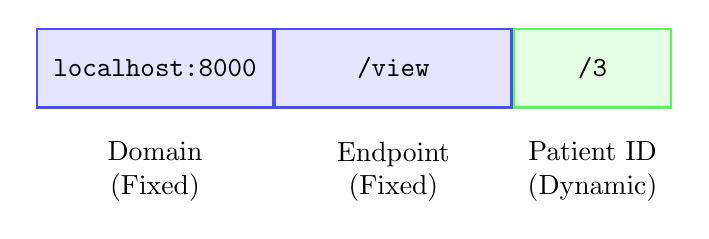
\begin{tikzpicture}[
    node distance=0.5cm,
    box/.style={rectangle, draw=blue!70, fill=blue!10, thick, minimum height=1cm, align=center}
]

\node[box, minimum width=3cm] (host) {\texttt{localhost:8000}};
\node[box, minimum width=3cm, right=0cm of host] (view) {\texttt{/view}};
\node[box, minimum width=2cm, right=0cm of view, fill=green!10, draw=green!70] (three) {\texttt{/3}};

\node[below=0.3cm of host, text width=3cm, align=center] {Domain\\(Fixed)};
\node[below=0.3cm of view, text width=1.5cm, align=center] {Endpoint\\(Fixed)};
\node[below=0.3cm of three, text width=2cm, align=center] {Patient ID\\(Dynamic)};

\end{tikzpicture}
\end{center}

\begin{itemize}[leftmargin=*]
    \item \texttt{localhost:8000} - \textbf{Cannot change} (domain)
    \item \texttt{/view} - \textbf{Cannot change} (endpoint path)
    \item \texttt{/3} - \textbf{Can change} (dynamic segment)
\end{itemize}

\subsection{The Dynamic Portion}

\begin{notebox}
The \texttt{/3} part is dynamic! Different clients can request different patient IDs:

\begin{itemize}[leftmargin=*]
    \item Client A requests: \texttt{/view/3}
    \item Client B requests: \texttt{/view/4}
    \item Client C requests: \texttt{/view/5}
\end{itemize}

This dynamic portion is called a \textbf{Path Parameter}.
\end{notebox}

\subsection{Purpose of Path Parameters}

Path parameters serve ONE primary purpose:

\begin{infobox}{Core Purpose}
\textbf{To locate and identify a SPECIFIC resource on the server}
\end{infobox}

In our example:
\begin{itemize}[leftmargin=*]
    \item The number \texttt{3} identifies which patient record to retrieve
    \item The server uses this to find that specific patient
    \item Only that patient's data is returned
\end{itemize}

\subsection{Common Use Cases for Path Parameters}

Path parameters are extremely useful for several operations:

\subsubsection{1. Retrieve Operations}

\begin{examplebox}{Viewing Specific Resources}
\textbf{Social Media Profile}:
\begin{verbatim}
GET /users/12345
\end{verbatim}

Retrieves profile of user with ID 12345 from all users in the database.
\end{examplebox}

\subsubsection{2. Update Operations}

\begin{examplebox}{Modifying Specific Resources}
\textbf{Updating Patient Weight}:
\begin{verbatim}
PUT /patient/P003
\end{verbatim}

Updates the record of patient P003 specifically, not all patients.
\end{examplebox}

\subsubsection{3. Delete Operations}

\begin{examplebox}{Removing Specific Resources}
\textbf{Deleting an Order}:
\begin{verbatim}
DELETE /orders/9876
\end{verbatim}

Deletes only order 9876, leaving other orders untouched.
\end{examplebox}

\begin{notebox}
\textbf{Key Observation}:

\vspace{0.5em}
Path parameters are used extensively in three CRUD operations:
\begin{itemize}[leftmargin=*]
    \item \textbf{Retrieve}: Get specific resource
    \item \textbf{Update}: Modify specific resource
    \item \textbf{Delete}: Remove specific resource
\end{itemize}

They help you work with ONE specific resource among many!
\end{notebox}

\newpage

% ========================
% SECTION 3: IMPLEMENTING PATH PARAMETERS
% ========================
\section{Implementing Path Parameters in FastAPI}

\subsection{Building the Endpoint}

Now let's create an endpoint that accepts a path parameter to view a specific patient.

\subsubsection{Step 1: Define the Route}

\begin{lstlisting}[language=Python, caption=Defining Route with Path Parameter]
@app.get('/patient/{patient_id}')
\end{lstlisting}

\textbf{Breaking down the route}:

\begin{itemize}[leftmargin=*]
    \item \texttt{/patient} - Fixed path segment
    \item \texttt{\{patient\_id\}} - Dynamic path parameter
    \item Curly braces \texttt{\{\}} indicate this is a variable
\end{itemize}

\begin{notebox}
The syntax \texttt{\{patient\_id\}} defines a path parameter. The name inside the braces becomes a variable that your function can access.
\end{notebox}

\subsubsection{Step 2: Create Handler Function}

\begin{lstlisting}[language=Python]
def view_patient(patient_id: str):
\end{lstlisting}

\textbf{Important points}:
\begin{itemize}[leftmargin=*]
    \item Function parameter name MUST match the route parameter name
    \item We specify the data type (\texttt{str} in this case)
    \item FastAPI automatically extracts the value from URL and passes it here
\end{itemize}

\begin{examplebox}{Why String Type?}
\textbf{Question}: Why is \texttt{patient\_id} a string?

\vspace{0.5em}
\textbf{Answer}: Looking at our \texttt{patients.json}:

\begin{lstlisting}[language=Python]
{
  "P001": {...},
  "P002": {...},
  "P003": {...}
}
\end{lstlisting}

Our patient IDs are formatted as "P001", "P002", etc. - these are strings, not integers!
\end{examplebox}

\subsubsection{Step 3: Implement Function Logic}

\begin{lstlisting}[language=Python, caption=Complete View Patient Function]
@app.get('/patient/{patient_id}')
def view_patient(patient_id: str):
    # Load all patient data
    data = load_data()
    
    # Check if patient ID exists
    if patient_id in data:
        # Return specific patient data
        return data[patient_id]
    
    # Return error if patient not found
    return {'error': 'patient not found'}
\end{lstlisting}

\subsection{Understanding the Flow}

\begin{center}
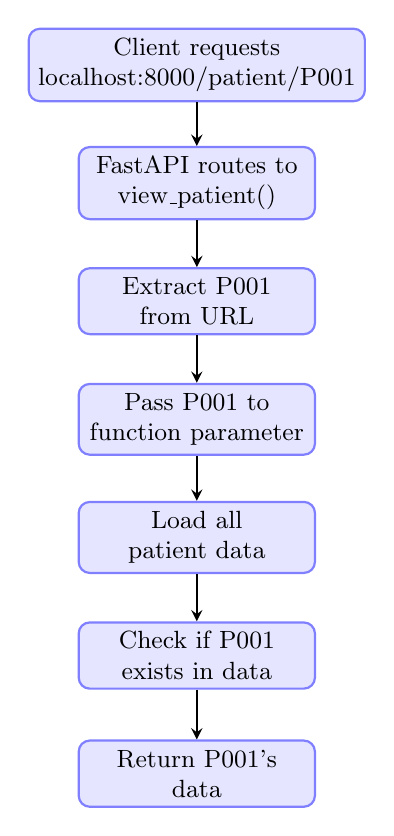
\begin{tikzpicture}[
    node distance=1.5cm,
    process/.style={rectangle, rounded corners, draw=blue!50, fill=blue!10, thick, minimum width=3cm, minimum height=0.8cm, font=\small, align=center},
    arrow/.style={->, >=stealth, thick}
]

\node[process] (request) {Client requests\\localhost:8000/patient/P001};
\node[process, below of=request] (route) {FastAPI routes to\\view\_patient()};
\node[process, below of=route] (extract) {Extract P001\\from URL};
\node[process, below of=extract] (pass) {Pass P001 to\\function parameter};
\node[process, below of=pass] (load) {Load all\\patient data};
\node[process, below of=load] (check) {Check if P001\\exists in data};
\node[process, below of=check] (return) {Return P001's\\data};

\draw[arrow] (request) -- (route);
\draw[arrow] (route) -- (extract);
\draw[arrow] (extract) -- (pass);
\draw[arrow] (pass) -- (load);
\draw[arrow] (load) -- (check);
\draw[arrow] (check) -- (return);

\end{tikzpicture}
\end{center}

\subsection{Testing the Endpoint}

\subsubsection{Method 1: Browser}

Simply navigate to:

\begin{cmdbox}
\begin{verbatim}
http://localhost:8000/patient/P001
http://localhost:8000/patient/P003
http://localhost:8000/patient/P005
\end{verbatim}
\end{cmdbox}

Each URL will return that specific patient's data!

\subsubsection{Method 2: Interactive Documentation}

Navigate to \texttt{http://localhost:8000/docs}

\begin{enumerate}[leftmargin=*]
    \item Find the \texttt{GET /patient/\{patient\_id\}} endpoint
    \item Click to expand it
    \item Notice it shows "patient\_id" as a \textbf{path parameter} (required)
    \item Click "Try it out"
    \item Enter "P001" in the patient\_id field
    \item Click "Execute"
    \item View the response below
\end{enumerate}

\begin{examplebox}{Response Example}
\textbf{Request}: \texttt{GET /patient/P001}

\vspace{0.5em}
\textbf{Response}:
\begin{lstlisting}[language=Python]
{
  "name": "Ananya Verma",
  "city": "Guwahati",
  "age": 28,
  "gender": "female",
  "height": 1.65,
  "weight": 90.0,
  "bmi": 33.06,
  "verdict": "Obese"
}
\end{lstlisting}
\end{examplebox}

\newpage

% ========================
% SECTION 4: ENHANCING WITH PATH() FUNCTION
% ========================
\section{Improving Code with the Path() Function}

\subsection{Current Problem with Documentation}

If you check the auto-generated documentation, you'll notice:
\begin{itemize}[leftmargin=*]
    \item It shows "patient\_id" is a path parameter
    \item It shows it's required
    \item But NO additional information is provided
\end{itemize}

\textbf{Why is this a problem?}

\begin{itemize}[leftmargin=*]
    \item Clients don't know what format the patient ID should be
    \item No examples are provided
    \item No description explains what this parameter does
    \item Makes API harder to use
\end{itemize}

\subsection{The Path() Function}

\begin{infobox}{What is Path()?}
\textbf{The Path() function in FastAPI is used to provide metadata, validation rules, and documentation hints for path parameters in your API endpoints.}
\end{infobox}

\subsection{Capabilities of Path()}

The Path() function allows you to:

\begin{center}
\begin{tabular}{|l|p{0.7\textwidth}|}
\hline
\textbf{Feature} & \textbf{Description} \\
\hline
Title & Add a title for the parameter \\
\hline
Description & Provide detailed explanation \\
\hline
Example & Show sample values \\
\hline
ge, gt, le, lt & Greater/less than validation (for numbers) \\
\hline
min\_length & Minimum string length \\
\hline
max\_length & Maximum string length \\
\hline
regex & Pattern matching validation \\
\hline
\end{tabular}
\end{center}

\subsection{Implementing Path() Function}

\subsubsection{Step 1: Import Path}

\begin{lstlisting}[language=Python]
from fastapi import FastAPI, Path
\end{lstlisting}

\subsubsection{Step 2: Use Path() in Function}

\begin{lstlisting}[language=Python, caption=Enhanced Path Parameter with Path()]
@app.get('/patient/{patient_id}')
def view_patient(
    patient_id: str = Path(
        ...,
        description="The ID of the patient in DB",
        example='P001'
    )
):
    data = load_data()
    
    if patient_id in data:
        return data[patient_id]
    
    return {'error': 'patient not found'}
\end{lstlisting}

\subsection{Understanding the Path() Parameters}

\subsubsection{The Ellipsis (...)}

\begin{lstlisting}[language=Python]
patient_id: str = Path(...)
\end{lstlisting}

\begin{infobox}{What does ... mean?}
The three dots \texttt{...} (ellipsis) indicate that this parameter is \textbf{required}.

\vspace{0.5em}
\textbf{Note}: All path parameters are required by default, but using \texttt{...} is considered best practice for clarity.
\end{infobox}

\subsubsection{Description}

\begin{lstlisting}[language=Python]
description="The ID of the patient in DB"
\end{lstlisting}

This text appears in the documentation, explaining what the parameter expects.

\subsubsection{Example}

\begin{lstlisting}[language=Python]
example='P001'
\end{lstlisting}

Provides a sample value that clients can see and use as reference.

\subsection{Additional Validation Options}

While not needed in our case, here are other validation options:

\begin{lstlisting}[language=Python, caption=Validation Examples]
# For numeric IDs
patient_id: int = Path(
    ...,
    ge=0,        # Greater than or equal to 0
    le=1000,     # Less than or equal to 1000
    description="Patient ID must be between 0 and 1000"
)

# For string length validation
patient_name: str = Path(
    ...,
    min_length=2,
    max_length=50,
    description="Patient name (2-50 characters)"
)

# For pattern matching
patient_code: str = Path(
    ...,
    regex="^P[0-9]{3}$",  # Must match P followed by 3 digits
    description="Patient code in format P001, P002, etc."
)
\end{lstlisting}

\subsection{Benefits After Adding Path()}

\subsubsection{Improved Documentation}

Navigate to \texttt{http://localhost:8000/docs} again:

\begin{examplebox}{Enhanced Documentation}
\textbf{Before Path()}:
\begin{itemize}[leftmargin=*]
    \item Shows: "patient\_id" (required)
    \item No other information
\end{itemize}

\textbf{After Path()}:
\begin{itemize}[leftmargin=*]
    \item Shows: "patient\_id" (required)
    \item Description: "The ID of the patient in DB"
    \item Example: "P001"
    \item Much clearer for API consumers!
\end{itemize}
\end{examplebox}

\begin{notebox}
\textbf{Key Takeaway}:

\vspace{0.5em}
Using the Path() function helps you create professional, well-documented APIs that are easy for clients to understand and use. It's a best practice in API development!
\end{notebox}

\newpage

% ========================
% SECTION 5: HTTP STATUS CODES
% ========================
\section{HTTP Status Codes: A Critical Concept}

Before we improve our code further, we need to understand an important concept: HTTP Status Codes.

\subsection{What Are HTTP Status Codes?}

\begin{infobox}{Definition}
\textbf{HTTP status codes are three-digit numbers returned by a web server to indicate the result of a client's request.}
\end{infobox}

\subsection{Understanding the Request-Response Flow}

Let's revisit how client-server communication works:

\begin{center}
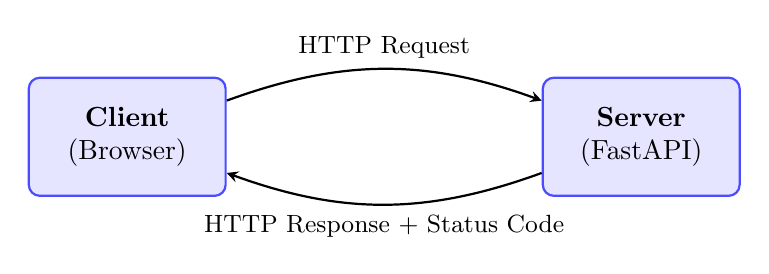
\begin{tikzpicture}[
    node distance=2.5cm,
    box/.style={rectangle, rounded corners, draw=blue!70, fill=blue!10, thick, minimum width=2.5cm, minimum height=1.5cm, align=center},
    arrow/.style={->, >=stealth, thick}
]

\node[box] (client) {\textbf{Client}\\(Browser)};
\node[box, right=4cm of client] (server) {\textbf{Server}\\(FastAPI)};

\draw[arrow, bend left=20] (client) to node[above, font=\small] {HTTP Request} (server);
\draw[arrow, bend left=20] (server) to node[below, font=\small] {HTTP Response + Status Code} (client);

\end{tikzpicture}
\end{center}

\textbf{The Communication Protocol}:

\begin{enumerate}[leftmargin=*]
    \item Client sends HTTP request to server
    \item Server processes the request
    \item Server prepares HTTP response
    \item \textbf{Server adds HTTP status code to response}
    \item Response sent back to client
\end{enumerate}

\begin{notebox}
\textbf{Important}: Every HTTP response includes a status code. This is a fundamental part of the HTTP protocol!
\end{notebox}

\subsection{Purpose of Status Codes}

Status codes tell the client:

\begin{itemize}[leftmargin=*]
    \item Was the request successful?
    \item If something went wrong, what type of error occurred?
    \item Does the client need to take any further action?
\end{itemize}

\subsection{Categories of Status Codes}

Status codes are grouped into 5 categories based on their first digit:

\begin{center}
\begin{tabular}{|c|l|p{0.5\textwidth}|}
\hline
\textbf{Range} & \textbf{Category} & \textbf{Meaning} \\
\hline
\textbf{2xx} & Success & Request was successful \\
\hline
\textbf{3xx} & Redirection & Further action needed \\
\hline
\textbf{4xx} & Client Error & Error on client's side \\
\hline
\textbf{5xx} & Server Error & Error on server's side \\
\hline
\end{tabular}
\end{center}

\begin{examplebox}{Quick Recognition}
\textbf{If you see a status code starting with}:

\begin{itemize}[leftmargin=*]
    \item \textbf{2}: Everything went well ✓
    \item \textbf{3}: Redirect or additional action needed
    \item \textbf{4}: You (client) did something wrong
    \item \textbf{5}: Server has a problem
\end{itemize}
\end{examplebox}

\subsection{Common HTTP Status Codes}

\subsubsection{2xx - Success Codes}

\begin{center}
\begin{tabular}{|l|l|p{0.5\textwidth}|}
\hline
\textbf{Code} & \textbf{Name} & \textbf{Meaning} \\
\hline
200 & OK & Request succeeded, response returned properly \\
\hline
201 & Created & Resource successfully created on server \\
\hline
204 & No Content & Success, but no data to return \\
\hline
\end{tabular}
\end{center}

\begin{examplebox}{200 OK - Most Common Success Code}
When you successfully retrieve data from an API:

\begin{verbatim}
GET /patient/P001

Response:
Status: 200 OK
Body: { "name": "Ananya Verma", "age": 28, ... }
\end{verbatim}

The 200 code tells you everything worked perfectly!
\end{examplebox}

\begin{examplebox}{201 Created - For POST Requests}
When you create a new patient record:

\begin{verbatim}
POST /patient

Response:
Status: 201 Created
Body: { "id": "P006", "message": "Patient created" }
\end{verbatim}

The 201 specifically indicates successful creation.
\end{examplebox}

\begin{examplebox}{204 No Content - For DELETE Requests}
When you delete a patient:

\begin{verbatim}
DELETE /patient/P001

Response:
Status: 204 No Content
Body: (empty)
\end{verbatim}

Success, but nothing to return since data was deleted.
\end{examplebox}

\subsubsection{4xx - Client Error Codes}

\begin{center}
\begin{tabular}{|l|l|p{0.45\textwidth}|}
\hline
\textbf{Code} & \textbf{Name} & \textbf{Meaning} \\
\hline
400 & Bad Request & Invalid request data, wrong format \\
\hline
401 & Unauthorized & Authentication required \\
\hline
403 & Forbidden & Logged in but not allowed \\
\hline
404 & Not Found & Resource doesn't exist \\
\hline
\end{tabular}
\end{center}

\begin{examplebox}{400 Bad Request}
Client sent wrong data format:

\begin{verbatim}
POST /patient
Body: { "age": "twenty-five" }  // Should be number, not string

Response:
Status: 400 Bad Request
Body: { "error": "Age must be a number" }
\end{verbatim}
\end{examplebox}

\begin{examplebox}{404 Not Found - Very Common!}
Client requested something that doesn't exist:

\begin{verbatim}
GET /patient/P999  // This patient doesn't exist

Response:
Status: 404 Not Found
Body: { "error": "Patient not found" }
\end{verbatim}

This is the famous "404 error" you've probably seen on websites!
\end{examplebox}

\subsubsection{5xx - Server Error Codes}

\begin{center}
\begin{tabular}{|l|l|p{0.5\textwidth}|}
\hline
\textbf{Code} & \textbf{Name} & \textbf{Meaning} \\
\hline
500 & Internal Server Error & Something went wrong on server \\
\hline
502 & Bad Gateway & Communication broken between servers \\
\hline
503 & Service Unavailable & Server down or overloaded \\
\hline
\end{tabular}
\end{center}

\subsection{Seeing Status Codes in Action}

Let's check our current endpoint in the documentation:

\begin{enumerate}[leftmargin=*]
    \item Go to \texttt{http://localhost:8000/docs}
    \item Find \texttt{GET /patient/\{patient\_id\}}
    \item Try it out with "P001"
    \item Execute
    \item Look at the response
\end{enumerate}

\begin{examplebox}{Successful Request}
\textbf{Request}: \texttt{GET /patient/P001}

\vspace{0.5em}
\textbf{Response}:
\begin{verbatim}
Status Code: 200
Body: {
  "name": "Ananya Verma",
  "city": "Guwahati",
  ...
}
\end{verbatim}

The 200 status code indicates success!
\end{examplebox}

\newpage

% ========================
% SECTION 6: THE PROBLEM WITH CURRENT CODE
% ========================
\section{Identifying the Problem: Incorrect Status Codes}

\subsection{Testing with Non-Existent Patient}

Let's test what happens when we request a patient that doesn't exist:

\begin{enumerate}[leftmargin=*]
    \item Go to \texttt{http://localhost:8000/docs}
    \item Open \texttt{GET /patient/\{patient\_id\}}
    \item Try it out with "P007" (doesn't exist in our database)
    \item Execute
    \item Observe the response
\end{enumerate}

\subsection{The Problem Revealed}

\begin{warningbox}
\textbf{What we see}:

\begin{verbatim}
Status Code: 200 OK

Response Body:
{
  "error": "patient not found"
}
\end{verbatim}

\textbf{The Problem}: Status code is 200 (Success), but we're returning an error!

\vspace{0.5em}
\textbf{Why this is wrong}:
\begin{itemize}[leftmargin=*]
    \item 200 means "request was successful"
    \item But the patient was NOT found
    \item This is misleading for API consumers
    \item Should be 404 (Not Found) instead
\end{itemize}
\end{warningbox}

\subsection{Why Status Codes Matter}

\begin{itemize}[leftmargin=*]
    \item API clients (apps, websites) rely on status codes
    \item They don't always read the response body
    \item Automated systems check status codes first
    \item 200 tells them "everything's fine" even when it's not
    \item Can cause bugs in client applications
\end{itemize}

\begin{examplebox}{Real-World Impact}
Imagine a mobile app using our API:

\begin{lstlisting}[language=Python]
# App code checking our API
response = fetch_patient("P999")

if response.status_code == 200:
    # App thinks everything is fine
    display_patient_info(response.data)
    # But data contains error message!
    # App might crash or show wrong info
\end{lstlisting}

Proper status codes prevent such issues!
\end{examplebox}

\subsection{The Solution: HTTPException}

FastAPI provides a special class to handle errors properly: \texttt{HTTPException}

\begin{infobox}{What is HTTPException?}
\textbf{HTTPException is a special built-in exception in FastAPI used to return custom HTTP error responses when something goes wrong in your API.}

\vspace{0.5em}
\textbf{Benefits}:
\begin{itemize}[leftmargin=*]
    \item Gracefully raise errors with proper status codes
    \item Include custom error messages
    \item Automatic error response formatting
    \item Better than returning error dictionaries
\end{itemize}
\end{infobox}

\subsection{Implementing HTTPException}

\subsubsection{Step 1: Import HTTPException}

\begin{lstlisting}[language=Python]
from fastapi import FastAPI, Path, HTTPException
\end{lstlisting}

\subsubsection{Step 2: Raise Exception Instead of Returning Error}

\begin{lstlisting}[language=Python, caption=Improved Code with HTTPException]
@app.get('/patient/{patient_id}')
def view_patient(
    patient_id: str = Path(
        ...,
        description="The ID of the patient in DB",
        example='P001'
    )
):
    data = load_data()
    
    if patient_id in data:
        return data[patient_id]
    
    # Instead of: return {'error': 'patient not found'}
    # We raise an HTTPException
    raise HTTPException(
        status_code=404,
        detail="Patient not found"
    )
\end{lstlisting}

\subsection{Understanding the Parameters}

\begin{center}
\begin{tabular}{|l|p{0.7\textwidth}|}
\hline
\textbf{Parameter} & \textbf{Description} \\
\hline
status\_code & The HTTP status code to return (404, 400, 500, etc.) \\
\hline
detail & The error message to include in response \\
\hline
\end{tabular}
\end{center}

\subsection{Testing the Improved Code}

\subsubsection{Test 1: Valid Patient}

\begin{cmdbox}
\begin{verbatim}
GET /patient/P001

Response:
Status Code: 200 OK
Body: { "name": "Ananya Verma", ... }
\end{verbatim}
\end{cmdbox}

✓ Works as expected!

\subsubsection{Test 2: Invalid Patient}

\begin{cmdbox}
\begin{verbatim}
GET /patient/P007

Response:
Status Code: 404 Not Found
Body: { "detail": "Patient not found" }
\end{verbatim}
\end{cmdbox}

✓ Now returns the correct 404 status code!

\begin{notebox}
\textbf{Going Forward}:

\vspace{0.5em}
From now on in this project, whenever something goes wrong, we'll use \texttt{HTTPException} with proper status codes instead of returning error dictionaries.

\vspace{0.5em}
This is a professional API development practice!
\end{notebox}

\subsection{Complete Updated Code}

\begin{lstlisting}[language=Python, caption=Complete Code with All Improvements]
from fastapi import FastAPI, Path, HTTPException
import json

app = FastAPI()

def load_data():    
    with open("patients.json", "r") as f:
        data = json.load(f)
    return data

@app.get("/")
def hello():
    return {"message": "Patient Management System API"}

@app.get("/about")  
def about():    
    return {"message": "A fully functional API for Patient Management"}

@app.get("/view")
def view(): 
    data = load_data()
    return data   

@app.get('/patient/{patient_id}')
def view_patient(
    patient_id: str = Path(
        ...,
        description="The ID of the patient in DB",
        example='P001'
    )
):
    data = load_data()
    
    if patient_id in data:
        return data[patient_id]  
    
    raise HTTPException(
        status_code=404,
        detail="Patient not found"
    )
\end{lstlisting}

\newpage

% ========================
% SECTION 7: QUERY PARAMETERS
% ========================
\section{Understanding Query Parameters}

\subsection{The New Requirement}

Let's introduce a new business requirement for our API.

\subsubsection{Current Situation}

We have the \texttt{/view} endpoint that returns ALL patients:

\begin{cmdbox}
\begin{verbatim}
GET /view

Returns: All 5 patients in chronological order
\end{verbatim}
\end{cmdbox}

\subsubsection{New Feature Request}

\hspace{1.5em}\textbf{Requirement}: Give users the option to view patients in SORTED order!

\vspace{0.5em}
\textbf{Specifically, allow sorting by}:
\begin{itemize}[leftmargin=*]
    \item Weight (ascending or descending)
    \item Height (ascending or descending)
    \item BMI (ascending or descending)
\end{itemize}

\textbf{Important}: This should be OPTIONAL!
\begin{itemize}[leftmargin=*]
    \item If user doesn't specify sorting → show data normally
    \item If user specifies sorting → show sorted data
\end{itemize}

\subsection{Why Not Path Parameters?}

\begin{warningbox}
\textbf{Question}: Can we use path parameters for this?

\vspace{0.5em}
\textbf{Answer}: NO! Here's why:

\begin{itemize}[leftmargin=*]
    \item Path parameters are REQUIRED
    \item Sorting is OPTIONAL
    \item Path parameters identify specific resources
    \item Sorting is a way to FILTER existing resources
    \item Path parameters change the endpoint structure
    \item We want to keep the same endpoint
\end{itemize}

We need something that's optional and doesn't change the endpoint → \textbf{Query Parameters}!
\end{warningbox}

\subsection{What Are Query Parameters?}

\begin{infobox}{Formal Definition}
\textbf{Query parameters are optional key-value pairs appended to the end of a URL, used to pass additional data to the server in an HTTP request.}

\vspace{0.5em}
They are typically employed for operations like:
\begin{itemize}[leftmargin=*]
    \item Filtering
    \item Sorting
    \item Searching
    \item Pagination
\end{itemize}

\textbf{WITHOUT altering the endpoint path itself!}
\end{infobox}

\subsection{Query Parameter Syntax}

\begin{examplebox}{URL Structure with Query Parameters}
\begin{verbatim}
http://localhost:8000/endpoint?key1=value1&key2=value2
\end{verbatim}

\textbf{Breaking it down}:

\begin{center}
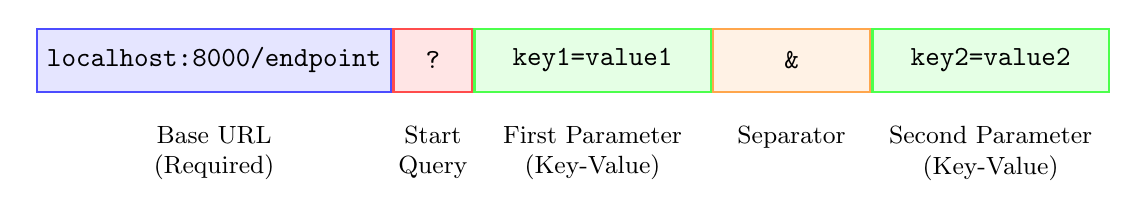
\begin{tikzpicture}[
    node distance=0.5cm,
    box/.style={rectangle, draw=blue!70, fill=blue!10, thick, minimum height=0.8cm, align=center}
]

\node[box, minimum width=4.5cm] (base) {\texttt{localhost:8000/endpoint}};
\node[box, minimum width=1cm, right=0cm of base, fill=red!10, draw=red!70] (q) {\texttt{?}};
\node[box, minimum width=3cm, right=0cm of q, fill=green!10, draw=green!70] (param1) {\texttt{key1=value1}};
\node[box, minimum width=2cm, right=0cm of param1, fill=orange!10, draw=orange!70] (amp) {\texttt{\&}};
\node[box, minimum width=3cm, right=0cm of amp, fill=green!10, draw=green!70] (param2) {\texttt{key2=value2}};

\node[below=0.3cm of base, text width=4.5cm, align=center, font=\small] {Base URL\\(Required)};
\node[below=0.3cm of q, text width=1cm, align=center, font=\small] {Start\\Query};
\node[below=0.3cm of param1, text width=3cm, align=center, font=\small] {First Parameter\\(Key-Value)};
\node[below=0.3cm of amp, text width=2cm, align=center, font=\small] {Separator};
\node[below=0.3cm of param2, text width=3cm, align=center, font=\small] {Second Parameter\\(Key-Value)};

\end{tikzpicture}
\end{center}
\end{examplebox}

\textbf{Key Elements}:

\begin{enumerate}[leftmargin=*]
    \item \textbf{? (Question Mark)}: Starts the query parameters section
    \item \textbf{key=value}: Each parameter as key-value pair
    \item \textbf{\& (Ampersand)}: Separates multiple parameters
\end{enumerate}

\subsection{Query Parameters vs Path Parameters}

\begin{center}
\begin{tabular}{|l|l|l|}
\hline
\textbf{Aspect} & \textbf{Path Parameters} & \textbf{Query Parameters} \\
\hline
Syntax & \texttt{/endpoint/\{value\}} & \texttt{/endpoint?key=value} \\
\hline
Required & Yes (always) & No (optional) \\
\hline
Purpose & Identify resource & Filter/modify results \\
\hline
Use case & Get specific item & Sort/filter items \\
\hline
Multiple values & Need multiple paths & Use \& separator \\
\hline
URL clarity & Part of path & After ? mark \\
\hline
\end{tabular}
\end{center}

\subsection{Real-World Examples}

\subsubsection{Example 1: E-commerce Search}

\begin{examplebox}{Product Search with Filters}
\begin{verbatim}
https://shop.com/products?category=electronics&price_max=500&sort=rating
\end{verbatim}

\textbf{Query Parameters}:
\begin{itemize}[leftmargin=*]
    \item \texttt{category=electronics}: Filter by category
    \item \texttt{price\_max=500}: Maximum price filter
    \item \texttt{sort=rating}: Sort by rating
\end{itemize}

All these are optional modifications to the /products endpoint!
\end{examplebox}

\subsubsection{Example 2: Social Media Feed}

\begin{examplebox}{Paginated Feed}
\begin{verbatim}
https://social.com/feed?page=2&limit=20&filter=friends
\end{verbatim}

\textbf{Query Parameters}:
\begin{itemize}[leftmargin=*]
    \item \texttt{page=2}: Show page 2
    \item \texttt{limit=20}: Show 20 items per page
    \item \texttt{filter=friends}: Show only friends' posts
\end{itemize}
\end{examplebox}

\subsection{Our Use Case: Patient Sorting}

For our Patient Management System, we'll use query parameters to enable sorting:

\begin{examplebox}{Patient Sorting URLs}
\textbf{Sort by BMI in descending order}:
\begin{verbatim}
http://localhost:8000/sort?sort_by=bmi&order=desc
\end{verbatim}

\textbf{Sort by height in ascending order}:
\begin{verbatim}
http://localhost:8000/sort?sort_by=height&order=asc
\end{verbatim}

\textbf{Just sort by weight (ascending by default)}:
\begin{verbatim}
http://localhost:8000/sort?sort_by=weight
\end{verbatim}

\textbf{Query Parameters}:
\begin{itemize}[leftmargin=*]
    \item \texttt{sort\_by}: Which field to sort on (weight/height/bmi)
    \item \texttt{order}: Sorting order (asc/desc) - OPTIONAL
\end{itemize}
\end{examplebox}

\newpage

% ========================
% SECTION 8: IMPLEMENTING QUERY PARAMETERS
% ========================
\section{Implementing Query Parameters in FastAPI}

\subsection{The Query() Function}

Just like we have \texttt{Path()} for path parameters, FastAPI provides \texttt{Query()} for query parameters.

\begin{infobox}{What is Query()?}
\textbf{Query() is a utility function provided by FastAPI to declare, validate, and document query parameters in your API endpoints.}

\vspace{0.5em}
\textbf{Capabilities}:
\begin{itemize}[leftmargin=*]
    \item Set default values
    \item Add validation rules (gt, lt, min\_length, max\_length)
    \item Provide metadata (title, description, examples)
    \item Make parameters optional or required
\end{itemize}
\end{infobox}

\subsection{Creating the Sort Endpoint}

\subsubsection{Step 1: Import Query}

\begin{lstlisting}[language=Python]
from fastapi import FastAPI, Path, HTTPException, Query
\end{lstlisting}

\subsubsection{Step 2: Define the Endpoint}

\begin{lstlisting}[language=Python, caption=Sort Endpoint with Query Parameters]
@app.get('/sort')
def sort_patients(
    sort_by: str = Query(
        ...,
        description='Sort on the basis of height, weight or BMI'
    ),
    order: str = Query(
        'asc',
        description="Sort in ascending or descending order"
    )
):
    # Implementation will follow
    pass
\end{lstlisting}

\subsection{Understanding the Parameters}

\subsubsection{Required Query Parameter}

\begin{lstlisting}[language=Python]
sort_by: str = Query(...)
\end{lstlisting}

\begin{itemize}[leftmargin=*]
    \item \texttt{...} (ellipsis) makes it REQUIRED
    \item User MUST provide this parameter
    \item If missing, FastAPI returns 422 error
\end{itemize}

\subsubsection{Optional Query Parameter with Default}

\begin{lstlisting}[language=Python]
order: str = Query('asc', ...)
\end{lstlisting}

\begin{itemize}[leftmargin=*]
    \item \texttt{'asc'} is the default value
    \item If user doesn't provide \texttt{order}, it defaults to 'asc'
    \item Makes this parameter OPTIONAL
\end{itemize}

\begin{notebox}
\textbf{Key Difference}:

\begin{itemize}[leftmargin=*]
    \item \texttt{Query(...)}: Parameter is required
    \item \texttt{Query('default\_value')}: Parameter is optional
\end{itemize}

This is how you control whether query parameters are mandatory or not!
\end{notebox}

\subsection{Implementing the Sorting Logic}

\subsubsection{Step 1: Define Valid Fields}

\begin{lstlisting}[language=Python]
def sort_patients(sort_by: str = Query(...), order: str = Query('asc')):
    # Define which fields can be sorted
    valid_fields = ['height', 'weight', 'bmi']
    
    # Validation will follow
\end{lstlisting}

\subsubsection{Step 2: Validate sort\_by Parameter}

\begin{lstlisting}[language=Python]
    # Check if sort_by is valid
    if sort_by not in valid_fields:
        raise HTTPException(
            status_code=400,
            detail=f'Invalid field, select from {valid_fields}'
        )
\end{lstlisting}

\textbf{Why 400?}
\begin{itemize}[leftmargin=*]
    \item 400 = Bad Request
    \item Client sent invalid data
    \item Client chose field that doesn't exist
    \item This is a client-side error
\end{itemize}

\subsubsection{Step 3: Validate order Parameter}

\begin{lstlisting}[language=Python]
    # Check if order is valid
    if order not in ['asc', 'desc']:
        raise HTTPException(
            status_code=400,
            detail='Invalid order, select from asc or desc'
        )
\end{lstlisting}

\subsubsection{Step 4: Load and Sort Data}

\begin{lstlisting}[language=Python]
    # Load all patient data
    data = load_data()
    
    # Determine sort order (True = descending, False = ascending)
    sort_order = True if order == 'desc' else False
    
    # Sort the data
    sorted_data = sorted(
        data.values(),
        key=lambda x: x[sort_by],
        reverse=sort_order
    )
    
    # Return sorted data
    return sorted_data
\end{lstlisting}

\subsection{Understanding the Sorting Code}

\subsubsection{Extracting Values}

\begin{lstlisting}[language=Python]
data.values()
\end{lstlisting}

\begin{itemize}[leftmargin=*]
    \item \texttt{data} is a dictionary \texttt{\{"P001": \{...\}, "P002": \{...\}\}}
    \item \texttt{.values()} extracts just the patient records
    \item Returns a list we can sort
\end{itemize}

\subsubsection{Lambda Function for Sorting Key}

\begin{lstlisting}[language=Python]
key=lambda x: x[sort_by]
\end{lstlisting}

\begin{itemize}[leftmargin=*]
    \item Lambda creates anonymous function
    \item \texttt{x} represents each patient dictionary
    \item \texttt{x[sort\_by]} extracts the sorting field
    \item If \texttt{sort\_by='bmi'}, it extracts BMI value
\end{itemize}

\subsubsection{Reverse Parameter}

\begin{lstlisting}[language=Python]
reverse=sort_order
\end{lstlisting}

\begin{itemize}[leftmargin=*]
    \item \texttt{reverse=False}: Ascending order (default)
    \item \texttt{reverse=True}: Descending order
\end{itemize}

\subsection{Complete Sort Function}

\begin{lstlisting}[language=Python, caption=Complete Sorting Implementation]
@app.get('/sort')
def sort_patients(
    sort_by: str = Query(
        ...,
        description='Sort on the basis of height, weight or BMI'
    ),
    order: str = Query(
        'asc',
        description="Sort in ascending or descending order"
    )
):
    # Define valid sorting fields
    valid_fields = ['height', 'weight', 'bmi']
    
    # Validate sort_by parameter
    if sort_by not in valid_fields:
        raise HTTPException(
            status_code=400,
            detail=f'Invalid field, select from {valid_fields}'
        )
    
    # Validate order parameter
    if order not in ['asc', 'desc']:
        raise HTTPException(
            status_code=400,
            detail='Invalid order, select from asc or desc'
        )
    
    # Load patient data
    data = load_data()
    
    # Determine sort order
    sort_order = True if order == 'desc' else False
    
    # Sort the data
    sorted_data = sorted(
        data.values(),
        key=lambda x: x[sort_by],
        reverse=sort_order
    )
    
    # Return sorted data
    return sorted_data
\end{lstlisting}

\newpage

% ========================
% SECTION 9: TESTING QUERY PARAMETERS
% ========================
\section{Testing the Sort Endpoint}

\subsection{Method 1: Direct URL Testing}

\subsubsection{Test 1: Sort by BMI in Descending Order}

\begin{cmdbox}
\begin{verbatim}
http://localhost:8000/sort?sort_by=bmi&order=desc
\end{verbatim}
\end{cmdbox}

\textbf{Expected Result}: Patients sorted from highest BMI to lowest

\begin{lstlisting}[language=Python]
[
  {
    "name": "Ananya Verma",
    "bmi": 33.06,    // Highest BMI first
    ...
  },
  {
    "name": "Neha Sinha",
    "bmi": 31.22,
    ...
  },
  {
    "name": "Ravi Mehta",
    "bmi": 27.76,
    ...
  },
  // ... continues in descending order
]
\end{lstlisting}

\subsubsection{Test 2: Sort by Height in Ascending Order}

\begin{cmdbox}
\begin{verbatim}
http://localhost:8000/sort?sort_by=height&order=asc
\end{verbatim}
\end{cmdbox}

\textbf{Expected Result}: Patients sorted from shortest to tallest

\subsubsection{Test 3: Sort by Weight (Default Ascending)}

\begin{cmdbox}
\begin{verbatim}
http://localhost:8000/sort?sort_by=weight
\end{verbatim}
\end{cmdbox}

\textbf{Note}: We didn't provide \texttt{order} parameter!

\vspace{0.5em}
\textbf{Result}: Since \texttt{order} has default value 'asc', it sorts in ascending order automatically.

\subsection{Method 2: Interactive Documentation}

\subsubsection{Testing Valid Request}

\begin{enumerate}[leftmargin=*]
    \item Navigate to \texttt{http://localhost:8000/docs}
    \item Find \texttt{GET /sort} endpoint
    \item Click to expand
    \item Click "Try it out"
    \item Notice TWO query parameters:
    \begin{itemize}
        \item \texttt{sort\_by}: Shows as required
        \item \texttt{order}: Shows with default value 'asc'
    \end{itemize}
    \item Enter "bmi" for sort\_by
    \item Enter "desc" for order
    \item Click "Execute"
    \item View response below
\end{enumerate}

\begin{examplebox}{Successful Response}
\textbf{Status Code}: 200 OK

\vspace{0.5em}
\textbf{Response Body}: Array of patient objects sorted by BMI in descending order
\end{examplebox}

\subsubsection{Testing Validation Errors}

\textbf{Test Invalid Field}:

\begin{enumerate}[leftmargin=*]
    \item Try it out again
    \item Enter "age" for sort\_by (not a valid field!)
    \item Enter "asc" for order
    \item Execute
\end{enumerate}

\begin{examplebox}{Validation Error Response}
\textbf{Status Code}: 400 Bad Request

\vspace{0.5em}
\textbf{Response Body}:
\begin{verbatim}
{
  "detail": "Invalid field, select from ['height', 'weight', 'bmi']"
}
\end{verbatim}

✓ Our validation is working!
\end{examplebox}

\textbf{Test Invalid Order}:

\begin{enumerate}[leftmargin=*]
    \item Enter "bmi" for sort\_by
    \item Enter "ascending" for order (should be 'asc' or 'desc'!)
    \item Execute
\end{enumerate}

\begin{examplebox}{Order Validation Error}
\textbf{Status Code}: 400 Bad Request

\vspace{0.5em}
\textbf{Response Body}:
\begin{verbatim}
{
  "detail": "Invalid order, select from asc or desc"
}
\end{verbatim}

✓ Validation catching invalid order values!
\end{examplebox}

\subsection{Verifying Optional Parameters}

\textbf{Test Without Order Parameter}:

\begin{enumerate}[leftmargin=*]
    \item Try it out
    \item Enter "weight" for sort\_by
    \item Leave order EMPTY or with default value
    \item Execute
\end{enumerate}

\textbf{Result}: Still works! Defaults to ascending order.

\begin{notebox}
This demonstrates the power of optional query parameters:
\begin{itemize}[leftmargin=*]
    \item Required parameters MUST be provided
    \item Optional parameters use defaults if not provided
    \item API remains flexible yet predictable
\end{itemize}
\end{notebox}

\newpage

% ========================
% SECTION 10: COMPLETE CODE REFERENCE
% ========================
\section{Complete Project Code}

\subsection{Final main.py}

\begin{lstlisting}[language=Python, caption=Complete Patient Management API with Parameters]
from fastapi import FastAPI, Path, HTTPException, Query
import json

app = FastAPI()

def load_data():    
    """Load patient data from JSON file"""
    with open("patients.json", "r") as f:
        data = json.load(f)
    return data

@app.get("/")
def hello():
    """Home endpoint"""
    return {"message": "Patient Management System API"}

@app.get("/about")  
def about():    
    """About endpoint"""
    return {
        "message": "A fully functional API for Patient Management System"
    }

@app.get("/view")
def view(): 
    """View all patients endpoint"""
    data = load_data()
    return data   

@app.get('/patient/{patient_id}')
def view_patient(
    patient_id: str = Path(
        ...,
        description="The ID of the patient in DB",
        example='P001'
    )
):
    """
    View specific patient by ID
    
    Path Parameter:
        patient_id: Unique identifier for the patient
    
    Returns:
        Patient data if found
    
    Raises:
        404: Patient not found
    """
    data = load_data()
    
    if patient_id in data:
        return data[patient_id]  
    
    raise HTTPException(
        status_code=404,
        detail="Patient not found"
    )

@app.get('/sort')
def sort_patients(
    sort_by: str = Query(
        ...,
        description='Sort on the basis of height, weight or BMI'
    ),
    order: str = Query(
        'asc',
        description="Sort in ascending or descending order"
    )
):
    """
    Sort patients by specified field
    
    Query Parameters:
        sort_by: Field to sort on (height/weight/bmi) - REQUIRED
        order: Sort order (asc/desc) - OPTIONAL, defaults to 'asc'
    
    Returns:
        List of patients sorted by specified criteria
    
    Raises:
        400: Invalid field or order value
    """
    # Define valid sorting fields
    valid_fields = ['height', 'weight', 'bmi']
    
    # Validate sort_by parameter
    if sort_by not in valid_fields:
        raise HTTPException(
            status_code=400,
            detail=f'Invalid field, select from {valid_fields}'
        )
    
    # Validate order parameter
    if order not in ['asc', 'desc']:
        raise HTTPException(
            status_code=400,
            detail='Invalid order, select from asc or desc'
        )
    
    # Load patient data
    data = load_data()
    
    # Determine sort order
    sort_order = True if order == 'desc' else False
    
    # Sort the data
    sorted_data = sorted(
        data.values(),
        key=lambda x: x[sort_by],
        reverse=sort_order
    )
    
    # Return sorted data
    return sorted_data
\end{lstlisting}

\subsection{API Endpoints Summary}

\begin{center}
\begin{tabular}{|l|l|p{0.45\textwidth}|}
\hline
\textbf{Endpoint} & \textbf{Method} & \textbf{Purpose} \\
\hline
/ & GET & Welcome message \\
\hline
/about & GET & API description \\
\hline
/view & GET & Get all patients \\
\hline
/patient/\{id\} & GET & Get specific patient (path param) \\
\hline
/sort & GET & Get sorted patients (query params) \\
\hline
\end{tabular}
\end{center}

\subsection{Project Structure}

\begin{cmdbox}
\begin{verbatim}
patient-management-api/
├── env/                    # Virtual environment
├── main.py                 # FastAPI application
├── patients.json           # Patient database
└── requirements.txt        # Python dependencies
\end{verbatim}
\end{cmdbox}

\newpage

% ========================
% SECTION 11: KEY CONCEPTS SUMMARY
% ========================
\section{Key Concepts Summary}

\subsection{Path Parameters Recap}

\begin{infobox}{Path Parameters - Quick Reference}
\textbf{Definition}: Dynamic segments of URL path to identify specific resources

\vspace{0.5em}
\textbf{Syntax}: \texttt{/endpoint/\{parameter\_name\}}

\vspace{0.5em}
\textbf{Characteristics}:
\begin{itemize}[leftmargin=*]
    \item Always REQUIRED
    \item Part of the URL path
    \item Used to identify specific resources
    \item Common in Retrieve, Update, Delete operations
\end{itemize}

\textbf{Example}:
\begin{verbatim}
/patient/P001  ← P001 is path parameter
\end{verbatim}
\end{infobox}

\subsection{Query Parameters Recap}

\begin{infobox}{Query Parameters - Quick Reference}
\textbf{Definition}: Optional key-value pairs at end of URL for filtering/modifying

\vspace{0.5em}
\textbf{Syntax}: \texttt{/endpoint?key1=value1\&key2=value2}

\vspace{0.5em}
\textbf{Characteristics}:
\begin{itemize}[leftmargin=*]
    \item Can be OPTIONAL or REQUIRED
    \item After ? in URL
    \item Used for filtering, sorting, pagination
    \item Don't change endpoint path
\end{itemize}

\textbf{Example}:
\begin{verbatim}
/sort?sort_by=bmi&order=desc  ← Query parameters
\end{verbatim}
\end{infobox}

\subsection{Path() vs Query() Functions}

\begin{center}
\begin{tabular}{|l|l|l|}
\hline
\textbf{Feature} & \textbf{Path()} & \textbf{Query()} \\
\hline
Used for & Path parameters & Query parameters \\
\hline
Required by default & Yes (always) & No (can set default) \\
\hline
Default values & Not applicable & Supported \\
\hline
Validation & Supported & Supported \\
\hline
Documentation & Enhanced & Enhanced \\
\hline
\end{tabular}
\end{center}

\subsection{HTTP Status Codes Reference}

\begin{center}
\begin{tabular}{|l|l|p{0.5\textwidth}|}
\hline
\textbf{Code} & \textbf{Name} & \textbf{When to Use} \\
\hline
\textbf{200} & OK & Successful GET/PUT/PATCH \\
\hline
\textbf{201} & Created & Successful POST (creation) \\
\hline
\textbf{204} & No Content & Successful DELETE \\
\hline
\textbf{400} & Bad Request & Invalid client data \\
\hline
\textbf{401} & Unauthorized & Authentication needed \\
\hline
\textbf{403} & Forbidden & Not allowed (even if authenticated) \\
\hline
\textbf{404} & Not Found & Resource doesn't exist \\
\hline
\textbf{500} & Server Error & Server-side problem \\
\hline
\end{tabular}
\end{center}

\subsection{When to Use Each Parameter Type}

\begin{examplebox}{Decision Guide}
\textbf{Use Path Parameters When}:
\begin{itemize}[leftmargin=*]
    \item Identifying a SPECIFIC resource
    \item Parameter is REQUIRED
    \item Working with single resource (retrieve/update/delete)
    \item Example: \texttt{/users/123}, \texttt{/orders/456}
\end{itemize}

\textbf{Use Query Parameters When}:
\begin{itemize}[leftmargin=*]
    \item Filtering MULTIPLE resources
    \item Parameter is OPTIONAL
    \item Sorting, searching, or paginating
    \item Example: \texttt{/products?category=books\&sort=price}
\end{itemize}
\end{examplebox}

\newpage

\section{Combining Both Parameter Types}

\begin{notebox}
\textbf{Can you use BOTH Path and Query Parameters in the same endpoint?}

\vspace{0.5em}
\textbf{Answer}: YES — this is not only valid, it is extremely common in real-world APIs.

\vspace{0.5em}
\textbf{Example Request}:
\begin{verbatim}
GET /users/{user_id}/posts?status=published&limit=10
\end{verbatim}

\begin{itemize}[leftmargin=*]
    \item \textbf{Path parameter}: \texttt{user\_id} — identifies \emph{which user}
    \item \textbf{Query parameters}: \texttt{status}, \texttt{limit} — filter that user’s posts
\end{itemize}

This pattern is widely used in REST APIs such as social media feeds, e-commerce orders, and dashboards.
\end{notebox}

\begin{lstlisting}[language=Python, caption=Using Path and Query Parameters Together]
from fastapi import FastAPI, Path, Query, HTTPException

app = FastAPI()

# Dummy database
posts_db = {
    "u101": [
        {"id": 1, "title": "FastAPI Basics", "status": "published"},
        {"id": 2, "title": "Draft Post", "status": "draft"},
        {"id": 3, "title": "Advanced FastAPI", "status": "published"}
    ]
}

@app.get("/users/{user_id}/posts")
def get_user_posts(
    user_id: str = Path(
        ...,
        description="Unique ID of the user",
        example="u101"
    ),
    status: str = Query(
        None,
        description="Filter posts by status (published or draft)",
        example="published"
    ),
    limit: int = Query(
        10,
        ge=1,
        le=50,
        description="Maximum number of posts to return",
        example=10
    )
):
    if user_id not in posts_db:
        raise HTTPException(
            status_code=404,
            detail="User not found"
        )

    posts = posts_db[user_id]

    if status:
        posts = [post for post in posts if post["status"] == status]

    return posts[:limit]
\end{lstlisting}

\begin{infobox}{How FastAPI Interprets This Endpoint}
\begin{itemize}[leftmargin=*]
    \item \texttt{user\_id} is extracted from the URL path
    \item \texttt{status} and \texttt{limit} are extracted from the query string
    \item Path parameters identify the resource
    \item Query parameters modify or filter the response
\end{itemize}

\vspace{0.5em}
This separation keeps URLs clean, readable, and scalable.
\end{infobox}

\begin{notebox}
\textbf{Golden Rule}:

\begin{itemize}[leftmargin=*]
\item Path parameters decide \emph{WHAT} resource you want.
\item Query parameters decide \emph{HOW} you want that resource.
\end{itemize}
\end{notebox}


\newpage

% ========================
% SECTION 12: BEST PRACTICES
% ========================
\section{Best Practices and Guidelines}

\subsection{Parameter Validation}

\begin{infobox}{Always Validate User Input}
\textbf{Never trust user input blindly!}

\begin{enumerate}[leftmargin=*]
    \item Use Path() and Query() for automatic validation
    \item Define acceptable values explicitly
    \item Return 400 status code for invalid input
    \item Provide clear error messages
\end{enumerate}
\end{infobox}

\begin{examplebox}{Good Validation Example}
\begin{lstlisting}[language=Python]
@app.get('/items')
def get_items(
    category: str = Query(
        ...,
        regex="^(books|electronics|clothing)$",
        description="Item category"
    ),
    min_price: float = Query(
        0,
        ge=0,
        le=10000,
        description="Minimum price filter"
    )
):
    # Input is validated before reaching here
    pass
\end{lstlisting}
\end{examplebox}

\subsection{Documentation Best Practices}

\begin{enumerate}[leftmargin=*]
    \item \textbf{Always add descriptions} to parameters
    \item \textbf{Provide examples} of valid values
    \item \textbf{Document error responses} in docstrings
    \item \textbf{Use type hints} consistently
    \item \textbf{Write clear function docstrings}
\end{enumerate}

\vspace{0.5em}
\begin{examplebox}{Well-Documented Endpoint}
\begin{lstlisting}[language=Python]
@app.get('/search')
def search_patients(
    name: str = Query(
        None,
        min_length=2,
        description="Search by patient name",
        example="John"
    ),
    min_age: int = Query(
        None,
        ge=0,
        le=150,
        description="Minimum age filter",
        example=18
    )
):
    """
    Search patients by name and/or age
    
    Query Parameters:
        name: Patient name (partial match)
        min_age: Minimum age filter
    
    Returns:
        List of matching patients
    """
    pass
\end{lstlisting}
\end{examplebox}

\subsection{Error Handling Best Practices}

\begin{warningbox}
\textbf{Use HTTPException for All Errors}

\vspace{0.5em}
\textbf{Don't}:
\begin{lstlisting}[language=Python]
return {"error": "Something went wrong"}  # Wrong
\end{lstlisting}

\textbf{Do}:
\begin{lstlisting}[language=Python]
raise HTTPException(
    status_code=400,
    detail="Something went wrong"
)  # Correct
\end{lstlisting}

\textbf{Why?}
\begin{itemize}[leftmargin=*]
    \item Proper HTTP status codes
    \item Consistent error format
    \item Better client experience
    \item Follows REST standards
\end{itemize}
\end{warningbox}

\subsection{Optional vs Required Parameters}

\begin{center}
\begin{tabular}{|p{0.5\textwidth}|p{0.5\textwidth}|}
\hline
\textbf{Required Parameter} & \textbf{Optional Parameter} \\
\hline
\begin{lstlisting}[language=Python]
param: str = Query(...)
# OR
param: str = Query()
\end{lstlisting}
& 
\begin{lstlisting}[language=Python]
param: str = Query("default")
# OR  
param: str = Query(None)
\end{lstlisting}
\\
\hline
Must be provided by client & Can be omitted \\
\hline
No default value & Has default value \\
\hline
FastAPI returns 422 if missing & Uses default if missing \\
\hline
\end{tabular}
\end{center}

\subsection{Naming Conventions}

\begin{infobox}{Parameter Naming Guidelines}
\textbf{Path Parameters}:
\begin{itemize}[leftmargin=*]
    \item Use singular nouns: \texttt{user\_id}, \texttt{product\_id}
    \item Describe the resource: \texttt{patient\_id}, not just \texttt{id}
    \item Use snake\_case
\end{itemize}

\textbf{Query Parameters}:
\begin{itemize}[leftmargin=*]
    \item Be descriptive: \texttt{sort\_by}, \texttt{filter\_status}
    \item Use snake\_case consistently
    \item Keep concise but clear
\end{itemize}
\end{infobox}

\newpage

% ========================
% SECTION 13: COMMON PITFALLS
% ========================
\section{Common Pitfalls and How to Avoid Them}

\subsection{Pitfall 1: Parameter Name Mismatch}

\begin{warningbox}
\textbf{Wrong}:
\begin{lstlisting}[language=Python]
@app.get('/patient/{patient_id}')
def view_patient(id: str):  # Names don't match!
    pass
\end{lstlisting}

\textbf{Error}: FastAPI won't find the parameter!

\vspace{0.5em}
\textbf{Correct}:
\begin{lstlisting}[language=Python]
@app.get('/patient/{patient_id}')
def view_patient(patient_id: str):  # Names match
    pass
\end{lstlisting}
\end{warningbox}

\subsection{Pitfall 2: Forgetting Question Mark in Query Parameters}

\begin{warningbox}
\textbf{Wrong URL}:
\begin{verbatim}
/sort&sort_by=bmi&order=desc  # Missing ?
\end{verbatim}

\textbf{Correct URL}:
\begin{verbatim}
/sort?sort_by=bmi&order=desc  # ✓ Has ?
\end{verbatim}

Remember: Query parameters ALWAYS start with \texttt{?}
\end{warningbox}

\subsection{Pitfall 3: Returning Wrong Status Codes}

\begin{warningbox}
\textbf{Wrong}:
\begin{lstlisting}[language=Python]
if not found:
    return {"error": "Not found"}  # Returns 200!
\end{lstlisting}

\textbf{Correct}:
\begin{lstlisting}[language=Python]
if not found:
    raise HTTPException(
        status_code=404,
        detail="Not found"
    )  # Returns 404
\end{lstlisting}
\end{warningbox}

\subsection{Pitfall 4: Not Validating User Input}

\begin{warningbox}
\textbf{Vulnerable Code}:
\begin{lstlisting}[language=Python]
@app.get('/sort')
def sort_patients(sort_by: str, order: str):
    # No validation!
    sorted_data = sorted(data.values(), key=lambda x: x[sort_by])
    # What if sort_by is invalid? KeyError!
\end{lstlisting}

\textbf{Safe Code}:
\begin{lstlisting}[language=Python]
@app.get('/sort')
def sort_patients(sort_by: str = Query(...), order: str = Query('asc')):
    valid_fields = ['height', 'weight', 'bmi']
    if sort_by not in valid_fields:
        raise HTTPException(status_code=400, detail="Invalid field")
    # Now safe to use sort_by
\end{lstlisting}
\end{warningbox}

\subsection{Pitfall 5: Confusing Path and Query Parameters}

\begin{examplebox}{When to Use Which?}
\textbf{Wrong Choice}:
\begin{lstlisting}[language=Python]
# Using path param for optional filtering
@app.get('/products/{category}/{min_price}/{max_price}')
# All become required, URL gets messy
\end{lstlisting}

\textbf{Better Choice}:
\begin{lstlisting}[language=Python]
# Using query params for optional filtering
@app.get('/products')
def get_products(
    category: str = Query(None),
    min_price: float = Query(None),
    max_price: float = Query(None)
):
    # All optional, clean URL
    pass
\end{lstlisting}
\end{examplebox}

\newpage

% ========================
% SECTION 14: TROUBLESHOOTING
% ========================
\section{Troubleshooting Guide}

\subsection{Issue: 422 Unprocessable Entity}

\textbf{Error Message}:
\begin{verbatim}
{
  "detail": [
    {
      "loc": ["query", "sort_by"],
      "msg": "field required",
      "type": "value_error.missing"
    }
  ]
}
\end{verbatim}

\textbf{Cause}: Required parameter not provided

\vspace{0.5em}
\textbf{Solution}:
\begin{itemize}[leftmargin=*]
    \item Ensure you're providing all required parameters
    \item Check parameter names match exactly
    \item For query params, use \texttt{?key=value} format
\end{itemize}

\subsection{Issue: Parameter Not Being Recognized}

\textbf{Symptoms}:
\begin{itemize}[leftmargin=*]
    \item Function receives None instead of value
    \item Parameter doesn't appear in docs
\end{itemize}

\textbf{Common Causes \& Solutions}:

\begin{enumerate}[leftmargin=*]
    \item \textbf{Name Mismatch}
    \begin{lstlisting}[language=Python]
# Wrong
@app.get('/user/{user_id}')
def get_user(id: str): 

# Correct
@app.get('/user/{user_id}')
def get_user(user_id: str): 
    \end{lstlisting}
    
    \item \textbf{Missing Type Annotation}
    \begin{lstlisting}[language=Python]
# Wrong
def get_user(user_id):  # No type

# Correct
def get_user(user_id: str):  # Has type
    \end{lstlisting}
\end{enumerate}

\subsection{Issue: Validation Not Working}

\textbf{Problem}: Invalid values passing through

\vspace{0.5em}
\textbf{Check}:
\begin{lstlisting}[language=Python]
# Are you using Path() or Query()?
@app.get('/endpoint')
def handler(param: str):  # No validation

@app.get('/endpoint')
def handler(param: str = Query(...)):  # With validation
\end{lstlisting}

\subsection{Issue: Status Codes Not Changing}

\textbf{Problem}: Always getting 200 even for errors

\vspace{0.5em}
\textbf{Cause}: Returning dictionaries instead of raising exceptions

\vspace{0.5em}
\textbf{Fix}:
\begin{lstlisting}[language=Python]
# Replace this:
return {"error": "Not found"}

# With this:
raise HTTPException(status_code=404, detail="Not found")
\end{lstlisting}

\newpage

% ========================
% SECTION 15: PRACTICE EXERCISES
% ========================
\section{Practice Exercises}

\subsection{Exercise 1: Add Age Filter}

\textbf{Task}: Create an endpoint to filter patients by age range

\vspace{0.5em}
\textbf{Requirements}:
\begin{itemize}[leftmargin=*]
    \item Endpoint: \texttt{GET /filter-by-age}
    \item Query parameters:
    \begin{itemize}
        \item \texttt{min\_age}: Minimum age (optional, default 0)
        \item \texttt{max\_age}: Maximum age (optional, default 150)
    \end{itemize}
    \item Return patients within age range
    \item Validate: min\_age $\leq$ max\_age
\end{itemize}

\textbf{Expected Usage}:
\begin{verbatim}
/filter-by-age?min_age=25&max_age=40
\end{verbatim}

\subsection{Exercise 2: Search by City}

\textbf{Task}: Add search functionality for patients by city

\vspace{0.5em}
\textbf{Requirements}:
\begin{itemize}[leftmargin=*]
    \item Endpoint: \texttt{GET /search-city}
    \item Query parameter: \texttt{city} (required)
    \item Return all patients from that city
    \item Case-insensitive search
    \item Return 404 if no patients found in that city
\end{itemize}

\subsection{Exercise 3: Update Patient Weight}

\textbf{Task}: Create endpoint to update a patient's weight

\vspace{0.5em}
\textbf{Requirements}:
\begin{itemize}[leftmargin=*]
    \item Endpoint: \texttt{PUT /patient/\{patient\_id\}/weight}
    \item Path parameter: \texttt{patient\_id}
    \item Query parameter: \texttt{new\_weight} (float, required)
    \item Update weight and recalculate BMI
    \item Return 404 if patient not found
    \item Return updated patient data
\end{itemize}

\subsection{Exercise 4: Pagination}

\textbf{Task}: Add pagination to view all patients

\vspace{0.5em}
\textbf{Requirements}:
\begin{itemize}[leftmargin=*]
    \item Endpoint: \texttt{GET /patients}
    \item Query parameters:
    \begin{itemize}
        \item \texttt{page}: Page number (default 1)
        \item \texttt{limit}: Items per page (default 10, max 100)
    \end{itemize}
    \item Return slice of patients based on pagination
    \item Include metadata: total\_count, page, limit
\end{itemize}

\textbf{Expected Response}:
\begin{lstlisting}[language=Python]
{
  "data": [ /* patient objects */ ],
  "page": 1,
  "limit": 10,
  "total_count": 5
}
\end{lstlisting}

\subsection{Solutions Approach}

\begin{notebox}
Try solving these exercises yourself first! They combine concepts from this session:

\begin{itemize}[leftmargin=*]
    \item Path parameters for resource identification
    \item Query parameters for filtering
    \item HTTPException for proper error handling
    \item Data validation
    \item Status codes
\end{itemize}

Solutions will use the same patterns we learned today!
\end{notebox}

\newpage

% ========================
% SECTION 17: QUICK REFERENCE
% ========================
\section{Quick Reference Guide}

\subsection{Command Reference}

\begin{tcolorbox}[colback=blue!5!white,colframe=blue!75!black,title=Essential Commands]
\begin{verbatim}
# Start server
uvicorn main:app --reload

# Access API
http://127.0.0.1:8000/

# Access documentation
http://127.0.0.1:8000/docs

# Test with path parameter
http://127.0.0.1:8000/patient/P001

# Test with query parameters
http://127.0.0.1:8000/sort?sort_by=bmi&order=desc
\end{verbatim}
\end{tcolorbox}

\subsection{Code Templates}

\subsubsection{Path Parameter Template}

\begin{lstlisting}[language=Python]
@app.get('/resource/{resource_id}')
def get_resource(
    resource_id: str = Path(
        ...,
        description="Resource identifier",
        example="123"
    )
):
    # Load data
    data = load_data()
    
    # Check if exists
    if resource_id in data:
        return data[resource_id]
    
    # Return 404
    raise HTTPException(
        status_code=404,
        detail="Resource not found"
    )
\end{lstlisting}

\subsubsection{Query Parameter Template}

\begin{lstlisting}[language=Python]
@app.get('/search')
def search(
    field: str = Query(
        ...,
        description="Field to search"
    ),
    value: str = Query(
        None,
        description="Search value"
    ),
    limit: int = Query(
        10,
        ge=1,
        le=100,
        description="Results limit"
    )
):
    # Validation
    if value is None:
        raise HTTPException(
            status_code=400,
            detail="Search value required"
        )
    
    # Search logic
    results = []  # Implement search
    
    return results[:limit]
\end{lstlisting}

\subsection{Import Statements}

\begin{lstlisting}[language=Python]
# All imports needed for this session
from fastapi import FastAPI, Path, Query, HTTPException
import json
\end{lstlisting}

\subsection{Status Code Quick Reference}

\begin{tcolorbox}[colback=green!5!white,colframe=green!75!black,title=Most Common Status Codes]
\begin{verbatim}
200 OK              - Successful GET/PUT/PATCH
201 Created         - Successful POST
204 No Content      - Successful DELETE
400 Bad Request     - Invalid client data
404 Not Found       - Resource doesn't exist
422 Unprocessable   - Validation error
500 Server Error    - Server problem
\end{verbatim}
\end{tcolorbox}

\subsection{URL Format Reference}

\begin{tcolorbox}[colback=yellow!5!white,colframe=orange!75!black,title=URL Patterns]
\begin{verbatim}
# Path parameter
/resource/{id}
Example: /patient/P001

# Query parameters
/resource?key1=value1&key2=value2
Example: /sort?sort_by=bmi&order=desc

# Combined (covered in future)
/resource/{id}?filter=value
Example: /patient/P001?include=history
\end{verbatim}
\end{tcolorbox}

\vfill

\begin{center}
\textit{End of FastAPI Path \& Query Parameters Guide}

\vspace{1em}

\textit{"The only way to do great work is to love what you do."}\\
\textit{— Steve Jobs}

\vspace{1em}

\textbf{Keep building, keep learning!}\\
Ready for the next session on POST requests and Pydantic models!
\end{center}

\end{document}